\documentclass[11pt,a4paper]{article}

% Packages
\usepackage[utf8]{inputenc}
\usepackage[T1]{fontenc}
\usepackage[margin=2.5cm]{geometry}
\usepackage{amsmath,amssymb}
\usepackage{enumitem}
\usepackage{listings}
\usepackage{xcolor}
\usepackage{tikz}
\usetikzlibrary{shapes.geometric, arrows, positioning, calc}
\usepackage{fancyhdr}
\usepackage{lastpage}
\usepackage{array}
\usepackage{tabularx}
\usepackage{booktabs}

% Code listing style
\definecolor{codebg}{RGB}{248,248,248}
\definecolor{codeframe}{RGB}{200,200,200}
\definecolor{codekw}{RGB}{0,0,180}
\definecolor{codecomment}{RGB}{0,128,0}
\definecolor{codestring}{RGB}{163,21,21}

\lstdefinestyle{pythonstyle}{
    language=Python,
    basicstyle=\ttfamily\small,
    keywordstyle=\color{codekw}\bfseries,
    commentstyle=\color{codecomment}\itshape,
    stringstyle=\color{codestring},
    backgroundcolor=\color{codebg},
    frame=single,
    rulecolor=\color{codeframe},
    numbers=left,
    numberstyle=\tiny\color{gray},
    numbersep=8pt,
    showstringspaces=false,
    showlines=true,
    breaklines=true,
    tabsize=4,
    xleftmargin=15pt,
    framexleftmargin=15pt,
}

\lstset{style=pythonstyle}

% Flowchart styles
\tikzstyle{startstop} = [rectangle, rounded corners, minimum width=2.5cm, minimum height=0.8cm, text centered, draw=black, fill=red!20]
\tikzstyle{process} = [rectangle, minimum width=2.5cm, minimum height=0.8cm, text centered, draw=black, fill=blue!15]
\tikzstyle{decision} = [diamond, aspect=2, minimum width=2cm, minimum height=0.8cm, text centered, draw=black, fill=green!15]
\tikzstyle{io} = [trapezium, trapezium left angle=70, trapezium right angle=110, minimum width=2cm, minimum height=0.8cm, text centered, draw=black, fill=orange!15]
\tikzstyle{arrow} = [thick,->,>=stealth]

% Header and footer
\pagestyle{fancy}
\fancyhf{}
\lhead{Python Programming -- Second Chance Exam}
\rhead{}
\cfoot{Page \thepage\ of \pageref{LastPage}}

% Points box
\newcommand{\pointsbox}[1]{\hfill\fbox{\textbf{#1 pts}}}

\begin{document}

% Title section
\begin{center}
  {\Large\bfseries Python Programming}\\[0.3cm]
  {\large Second Chance Exam}\\[0.3cm]
  {\normalsize 23.01.2026}\\[0.5cm]

  \vfil
  \textbf{Name:} \hrulefill
  \vfil

\end{center}

\vspace{0.5cm}

\noindent\textbf{Instructions:}
\begin{itemize}[noitemsep]
  \item Time allowed: \textbf{2 hours}
  \item Total points: \textbf{60 points}
  \item No aids (no notes, no electronic devices)
\end{itemize}

\vspace{0.3cm}

\noindent\textbf{Points Summary:}
\begin{center}
  \begin{tabular}{|c|c|c|}
    \hline
    \textbf{Question} & \textbf{Max Points} & \textbf{Score} \\
    \hline
    1                 & 4                   &                \\
    \hline
    2                 & 6                   &                \\
    \hline
    3                 & 5                   &                \\
    \hline
    4                 & 7                   &                \\
    \hline
    5                 & 8                   &                \\
    \hline
    6                 & 6                   &                \\
    \hline
    7                 & 9                   &                \\
    \hline
    8                 & 15                  &                \\
    \hline
    \textbf{Total}    & \textbf{60}         &                \\
    \hline
  \end{tabular}
\end{center}

\newpage

%==============================================================================
% QUESTION 1: Multiple Choice (Fundamentals & Types)
%==============================================================================
\section*{Question 1: Multiple Choice \pointsbox{4}}

\textit{Circle the correct answer for each question. Each correct answer is worth 1 point.}

\vspace{0.4cm}

\begin{enumerate}[label=\textbf{1.\arabic*}]
  \item What is the output of the following expression?
        \begin{lstlisting}[numbers=none]
result = 23 % 6
print(result)
    \end{lstlisting}
        \begin{enumerate}[label=\Alph*)]
          \item \texttt{3}
          \item \texttt{5}
          \item \texttt{4}
          \item \texttt{6}
        \end{enumerate}

        \vspace{0.5cm}

  \item Which of the following is an \textbf{immutable} data structure in Python?
        \begin{enumerate}[label=\Alph*)]
          \item \texttt{list}
          \item \texttt{dict}
          \item \texttt{str}
          \item \texttt{set}
        \end{enumerate}

        \vspace{0.5cm}

  \item What will \texttt{type("42")} return?
        \begin{enumerate}[label=\Alph*)]
          \item \texttt{<class 'int'>}
          \item \texttt{<class 'float'>}
          \item \texttt{<class 'str'>}
          \item \texttt{<class 'number'>}
        \end{enumerate}

        \vspace{0.5cm}

  \item What is the correct way to check if a key exists in a dictionary?
        \begin{enumerate}[label=\Alph*)]
          \item \texttt{if key in dict:}
          \item \texttt{if key == dict:}
          \item \texttt{if dict.has\_key(key):}
          \item \texttt{if key(dict):}
        \end{enumerate}
\end{enumerate}

\newpage

%==============================================================================
% QUESTION 2: Predict the Output
%==============================================================================
\section*{Question 2: Predict the Output \pointsbox{6}}

\textit{For each code snippet, write exactly what will be printed. Be precise with spacing and format.}

\vspace{0.4cm}

\begin{enumerate}[label=\textbf{2.\arabic*}]
  \item \textbf{(1 pt)}
        \begin{lstlisting}
fruits = ["apple", "banana", "cherry", "date"]
print(fruits[0:2])
print(fruits[-1])
    \end{lstlisting}
        \textbf{Output:}
        \vfil

  \item \textbf{(2 pts)}
        \begin{lstlisting}
a = 10
b = 20
a, b = a + b, a - b
print(f"a={a}, b={b}")
    \end{lstlisting}
        \textbf{Output:}


        \newpage
  \item \textbf{(1 pt)}
        \begin{lstlisting}
scores = {"Alice": 90, "Bob": 75, "Charlie": 85}
for name in scores:
    if scores[name] >= 80:
        print(name, end=" ")
    \end{lstlisting}
        \textbf{Output:}
        \vfil

  \item \textbf{(2 pts)}
        \begin{lstlisting}
def modify(lst):
    lst[0] = 999
    lst = [0, 0, 0]
    return lst

original = [1, 2, 3]
result = modify(original)
print(original)
print(result)
    \end{lstlisting}
        \textbf{Output:}
        \vfil
\end{enumerate}

\newpage

%==============================================================================
% QUESTION 3: Find the Errors
%==============================================================================
\section*{Question 3: Find and Fix the Errors \pointsbox{5}}

\textit{Each code snippet contains one or more errors. Identify each error and write the corrected line(s). Explain briefly what was wrong.}

\vspace{0.4cm}

\begin{enumerate}[label=\textbf{3.\arabic*}]
  \item \textbf{(1 pt)} The following code should calculate the square of a number but contains an error:
        \begin{lstlisting}
x = 7
square = x ** 2
print(square
    \end{lstlisting}
        \textbf{Error:}
        \vspace{1cm}

        \textbf{Correction:}
        \vspace{1.5cm}

  \item \textbf{(2 pts)} The following function should count the number of characters in a string:
        \begin{lstlisting}
def count_chars(text)
    count = 0
    for char in text
        count += 1
    return count
    \end{lstlisting}
        \textbf{Errors (list all):}
        \vspace{2cm}

        \textbf{Corrected code:}
        \vspace{3cm}

  \item \textbf{(2 pts)} The following class definition has an error:
        \begin{lstlisting}
class Book:
    def __init__(title, author):
        self.title = title
        self.author = author

book1 = Book("1984", "George Orwell")
    \end{lstlisting}
        \textbf{Error:}
        \vspace{1cm}

        \textbf{Correction:}
        \vspace{1.5cm}
\end{enumerate}

\newpage

%==============================================================================
% QUESTION 4: Flowchart to Code
%==============================================================================
\section*{Question 4: Flowchart to Python Code \pointsbox{7}}

\textit{Study the following flowchart and write the equivalent Python code. The flowchart calculates the sum of numbers from 1 to n.}

\vspace{0.4cm}

\begin{center}
  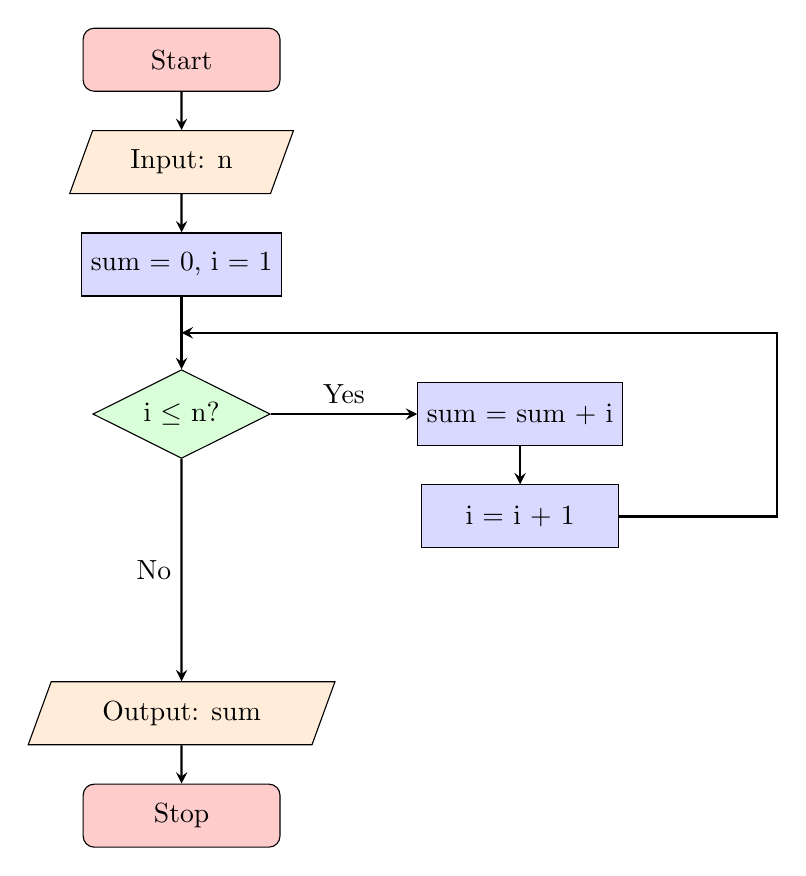
\begin{tikzpicture}[node distance=1.3cm]
    \node (start) [startstop] {Start};
    \node (input) [io, below of=start] {Input: n};
    \node (init) [process, below of=input] {sum = 0, i = 1};
    \node (check) [decision, below of=init, yshift=-0.6cm] {i $\leq$ n?};
    \node (addsum) [process, right of=check, xshift=3cm] {sum = sum + i};
    \node (increment) [process, below of=addsum] {i = i + 1};
    \node (output) [io, below of=check, yshift=-2.5cm] {Output: sum};
    \node (stop) [startstop, below of=output] {Stop};

    \draw [arrow] (start) -- (input);
    \draw [arrow] (input) -- (init);
    \draw [arrow] (init) -- (check);
    \draw [arrow] (check) -- node[anchor=south] {Yes} (addsum);
    \draw [arrow] (addsum) -- (increment);
    % Loop back
    \coordinate (loopback) at ($(init.south)!0.5!(check.north)$);
    \draw [arrow] (increment.east) -- +(2,0) |- (loopback);
    \draw [arrow] (check) -- node[anchor=east] {No} (output);
    \draw [arrow] (output) -- (stop);
  \end{tikzpicture}
\end{center}

\vspace{0.3cm}
\textbf{Hint:} Trace through the flowchart with \texttt{n = 5} to understand what it does before writing the code.

\vspace{0.2cm}
\textbf{Reminder:} The flowchart uses comparison operators and increments in a loop.

\vspace{0.3cm}
\textbf{Write the Python code that implements this flowchart on the next page.}

\newpage

\textbf{Question 4 -- Answer Space:}

\vfill

\newpage

%==============================================================================
% QUESTION 5: Code to Flowchart
%==============================================================================
\section*{Question 5: Python Code to Flowchart \pointsbox{8}}

\textit{Given the following Python code, draw a flowchart that represents its logic. Use proper flowchart symbols (oval for start/stop, rectangle for process, diamond for decision, parallelogram for input/output).}

\vspace{0.4cm}

\begin{lstlisting}
def classify_number(num):
    if num < 0:
        category = "Negative"
    elif num == 0:
        category = "Zero"
    elif num < 100:
        category = "Small Positive"
    else:
        category = "Large Positive"
    
    if num % 2 == 0:
        parity = "Even"
    else:
        parity = "Odd"
    
    return category, parity
\end{lstlisting}

\vspace{0.3cm}
\textbf{Draw your flowchart on the next page.}

\newpage

\textbf{Question 5 -- Answer Space:}

\vfill

\newpage

%==============================================================================
% QUESTION 6: Data Structures
%==============================================================================
\section*{Question 6: Data Structures \pointsbox{6}}

\begin{enumerate}[label=\textbf{6.\arabic*}]
  \item \textbf{(2 pts)} Given the following list of products, write Python code to:
        \begin{lstlisting}[numbers=none]
products = {
    "laptop": 1200,
    "mouse": 25,
    "keyboard": 75,
    "monitor": 350
}
    \end{lstlisting}

        \begin{enumerate}[label=\alph*)]
          \item Add a new product ``headphones'' with price 150:
                \vspace{1.5cm}

          \item Print all products that cost more than 100:
                \vspace{2.5cm}
        \end{enumerate}

  \item \textbf{(2 pts)} What is the difference between a \textbf{set} and a \textbf{list}? Give one practical use case for each.
        \vspace{3.5cm}

  \item \textbf{(2 pts)} What will be the contents of \texttt{numbers} after executing the following code?
        \begin{lstlisting}
numbers = [1, 2, 3, 2, 1, 4, 5, 4]
unique_numbers = set(numbers)
unique_numbers.add(6)
unique_numbers.remove(2)
    \end{lstlisting}
        \textbf{Answer:}
        \vspace{1.5cm}
\end{enumerate}

\newpage

%==============================================================================
% QUESTION 7: Functions
%==============================================================================
\section*{Question 7: Functions \pointsbox{9}}

\begin{enumerate}[label=\textbf{7.\arabic*}]
  \item \textbf{(3 pts)} Complete the following function that takes a list of numbers and returns a new list containing only the odd numbers:
        \begin{lstlisting}
def filter_odd(numbers):
    # Your code here
 
 
 
 
 
 
 
 
 
 
 
 
 
 

    \end{lstlisting}
\vfil
  \item \textbf{(3 pts)} Explain the difference between these two functions. What will each print when called?
        \begin{lstlisting}
def process_a(value):
    return value + 10

def process_b(value):
    print(value + 10)

result_a = process_a(5)
result_b = process_b(5)
print(f"result_a: {result_a}")
print(f"result_b: {result_b}")
    \end{lstlisting}
        \textbf{Explanation and Output:}
        \vfil

        \newpage
  \item \textbf{(3 pts)} Write a function called \texttt{count\_consonants} that takes a string and returns the number of consonants (all letters except a, e, i, o, u) in it. The function should work for both uppercase and lowercase letters.

        \textbf{Example:} \texttt{count\_consonants("Python")} should return \texttt{4}

        \vspace{7cm}
\end{enumerate}

\newpage

%==============================================================================
% QUESTION 8: Object-Oriented Programming
%==============================================================================
\section*{Question 8: Object-Oriented Programming \pointsbox{15}}

\begin{enumerate}[label=\textbf{8.\arabic*}]
  \item \textbf{(4 pts)} What is the output of the following code? Explain why.
        \begin{lstlisting}
class BankAccount:
    def __init__(self, owner, balance):
        self.owner = owner
        self._balance = balance
    
    @property
    def balance(self):
        return self._balance
    
    @balance.setter
    def balance(self, amount):
        if amount < 0:
            print("Cannot set negative balance!")
            return
        self._balance = amount
    
    def deposit(self, amount):
        self._balance += amount
        return self._balance

account = BankAccount("Alice", 1000)
account.balance = 500
print(account.balance)
account.balance = -200
print(account.balance)
account.deposit(150)
print(account.balance)
    \end{lstlisting}
        \textbf{Output:}
        \vspace{2.5cm}

        \textbf{What is the purpose of the balance setter validation in this code?}
        \vspace{2cm}

        \newpage
  \item \textbf{(4 pts)} The following code has a common OOP bug. Identify the bug, explain why it happens, and write the corrected code.
        \begin{lstlisting}
class Counter:
    count = 0
    
    def __init__(self, name):
        self.name = name
    
    def increment(self):
        self.count += 1

c1 = Counter("First")
c2 = Counter("Second")
c1.increment()
c1.increment()
c2.increment()
print(f"c1.count: {c1.count}")
print(f"c2.count: {c2.count}")
    \end{lstlisting}
        \textbf{What is the bug and why does it happen?}
        \vspace{2.5cm}

        \textbf{Write the corrected \texttt{\_\_init\_\_} method:}
        \vspace{4cm}

        \newpage

  \item \textbf{(4 pts)} Complete the \texttt{Library} class with proper encapsulation. The books list should be private (use \texttt{\_books}) and only accessible through a property that returns a copy (to prevent external modification).
        \begin{lstlisting}
class Library:
    def __init__(self, name):
        self.name = name
        # TODO: Initialize private _books as empty list
 
 

    @property
    def books(self):
        # TODO: Return a COPY of the books list
 
 

    @property
    def total_books(self):
        # TODO: Return number of books
 
 

    def add_book(self, title):
        # TODO: Add book only if not already in library
        # Return True if added, False if duplicate
 
 
 
 
 
 

    def remove_book(self, title):
        # TODO: Remove book if exists
        # Return True if removed, False if not found
 
 
 
 
 
 
    \end{lstlisting}

        \newpage
  \item \textbf{(3 pts)} Consider the following inheritance hierarchy:
        \begin{lstlisting}
class Vehicle:
    def __init__(self, brand):
        self.brand = brand
    
    def description(self):
        return f"Vehicle: {self.brand}"

class Car(Vehicle):
    def __init__(self, brand, doors):
        super().__init__(brand)
        self.doors = doors
    
    def description(self):
        base = super().description()
        return f"{base}, Doors: {self.doors}"

class SportsCar(Car):
    def description(self):
        base = super().description()
        return f"{base}, Type: Performance"

car = SportsCar("Ferrari", 2)
print(car.description())
print(isinstance(car, Vehicle))
    \end{lstlisting}

        \begin{enumerate}[label=\alph*)]
          \item What will be printed?
                \vspace{1.5cm}

          \item Trace the \texttt{super().description()} calls: which methods are called and in what order when \texttt{car.description()} executes?
                \vspace{2cm}

          \item What would happen if \texttt{SportsCar} had its own \texttt{\_\_init\_\_} method that didn't call \texttt{super()}? Explain briefly.
                \vspace{2cm}
        \end{enumerate}
\end{enumerate}

\vfill

\begin{center}
  \rule{8cm}{0.4pt}\\[0.3cm]
  \textbf{End of Exam}\\[0.2cm]
  \textit{Good luck!}
\end{center}

\end{document}
